% Options for packages loaded elsewhere
\PassOptionsToPackage{unicode}{hyperref}
\PassOptionsToPackage{hyphens}{url}
\PassOptionsToPackage{dvipsnames,svgnames,x11names}{xcolor}
\PassOptionsToPackage{space}{xeCJK}
\documentclass[
  10pt,
]{article}
\usepackage{xcolor}
\usepackage[margin=0.65in]{geometry}
\usepackage{amsmath,amssymb}
\setcounter{secnumdepth}{-\maxdimen} % remove section numbering
\usepackage{iftex}
\ifPDFTeX
  \usepackage[T1]{fontenc}
  \usepackage[utf8]{inputenc}
  \usepackage{textcomp} % provide euro and other symbols
\else % if luatex or xetex
  \usepackage{unicode-math} % this also loads fontspec
  \defaultfontfeatures{Scale=MatchLowercase}
  \defaultfontfeatures[\rmfamily]{Ligatures=TeX,Scale=1}
\fi
\usepackage{lmodern}
\ifPDFTeX\else
  % xetex/luatex font selection
  \setmainfont[]{Arial}
  \setmonofont[]{Consolas}
  \ifXeTeX
    \usepackage{xeCJK}
    \setCJKmainfont[]{Microsoft YaHei}
  \fi
  \ifLuaTeX
    \usepackage[]{luatexja-fontspec}
    \setmainjfont[]{Microsoft YaHei}
  \fi
\fi
% Use upquote if available, for straight quotes in verbatim environments
\IfFileExists{upquote.sty}{\usepackage{upquote}}{}
\IfFileExists{microtype.sty}{% use microtype if available
  \usepackage[]{microtype}
  \UseMicrotypeSet[protrusion]{basicmath} % disable protrusion for tt fonts
}{}
\makeatletter
\@ifundefined{KOMAClassName}{% if non-KOMA class
  \IfFileExists{parskip.sty}{%
    \usepackage{parskip}
  }{% else
    \setlength{\parindent}{0pt}
    \setlength{\parskip}{6pt plus 2pt minus 1pt}}
}{% if KOMA class
  \KOMAoptions{parskip=half}}
\makeatother
\usepackage{longtable,booktabs,array}
\usepackage{calc} % for calculating minipage widths
% Correct order of tables after \paragraph or \subparagraph
\usepackage{etoolbox}
\makeatletter
\patchcmd\longtable{\par}{\if@noskipsec\mbox{}\fi\par}{}{}
\makeatother
% Allow footnotes in longtable head/foot
\IfFileExists{footnotehyper.sty}{\usepackage{footnotehyper}}{\usepackage{footnote}}
\makesavenoteenv{longtable}
\usepackage{graphicx}
\makeatletter
\newsavebox\pandoc@box
\newcommand*\pandocbounded[1]{% scales image to fit in text height/width
  \sbox\pandoc@box{#1}%
  \Gscale@div\@tempa{\textheight}{\dimexpr\ht\pandoc@box+\dp\pandoc@box\relax}%
  \Gscale@div\@tempb{\linewidth}{\wd\pandoc@box}%
  \ifdim\@tempb\p@<\@tempa\p@\let\@tempa\@tempb\fi% select the smaller of both
  \ifdim\@tempa\p@<\p@\scalebox{\@tempa}{\usebox\pandoc@box}%
  \else\usebox{\pandoc@box}%
  \fi%
}
% Set default figure placement to htbp
\def\fps@figure{htbp}
\makeatother
\setlength{\emergencystretch}{3em} % prevent overfull lines
\providecommand{\tightlist}{%
  \setlength{\itemsep}{0pt}\setlength{\parskip}{0pt}}
\usepackage{bookmark}
\IfFileExists{xurl.sty}{\usepackage{xurl}}{} % add URL line breaks if available
\urlstyle{same}
\hypersetup{
  colorlinks=true,
  linkcolor={Maroon},
  filecolor={Maroon},
  citecolor={Blue},
  urlcolor={blue},
  pdfcreator={LaTeX via pandoc}}

\author{}
\date{}

\usepackage{float}
\usepackage{needspace}
\setCJKmonofont{Microsoft YaHei}
\Urlmuskip=0mu plus 2mu\relax
\renewcommand{\figurename}{图}
\begin{document}

\section{数据扩展与退化增强：实验结果分析}\label{ux6570ux636eux6269ux5c55ux4e0eux9000ux5316ux589eux5f3aux5b9eux9a8cux7ed3ux679cux5206ux6790}

2026年11月13日 · \href{experimental-analysis.en.md}{English} ·
\href{experimental-analysis.zh.pdf}{中文 PDF}

扩展数据提高了 KEH 和 LAG 来源的青光眼图像排序表现，AIROGS 和 ODIR
来源的表现下降。50\%
退化增强提高了合成失焦图像的排序表现，并减少误报，同时增加部分阳性漏诊。12
张真实低质量开发阳性图像在三个扩展方案下均被检出，退化增强在这组图像上没有额外检出。

本文承接同日的\href{../data-review/data-and-degradation-review.zh.md}{数据与方法审查}和\href{../training-results/training-results.zh.md}{训练结果报告}，进一步分析来源差异、实际采样次数、权重选择以及真实低质量图像的标签分布。这些分析为下一轮控制实验提供依据。

\subsection{数据、模型与比较方法}\label{ux6570ux636eux6a21ux578bux4e0eux6bd4ux8f83ux65b9ux6cd5}

四个方案均使用 EfficientNet-B0、相同初始化和随机种子 20261113，各完成
1,200 次有效优化更新。原数据方案使用 10,338 张训练图像；三个扩展方案使用
15,480 张。30\% 和 50\%
表示采样图像应用混合退化增强的概率。阳性保留各来源的定义，包括青光眼诊断和
AIROGS 的青光眼转诊标签，因此结果按来源分析。模型验证集含 2,046
张图像，其中阳性 823 张；规则开发集含 2,053 张，其中阳性 814
张。模型验证集用于选择权重和设定来源阈值，规则开发集用于拟定人工复核规则及本文的结果分析。最终测试将在模型和复核规则确定后执行。

训练报告记录的是验证指标最高时选中的权重：原数据、30\% 退化和 50\%
退化均选中第 1,200 次更新，扩展无退化选中第 300
次更新。本文主要使用四组第 1,200
次更新权重，使比较具有相同更新预算；选中权重的结果另存于\href{analysis.json}{分析数据}。一轮训练表示完整遍历训练集，优化更新表示处理一个批次后调整模型参数，本轮预算按更新次数设定。

95\% 区间通过 4,000
次配对自助重采样计算：每次抽取完整关联组，同一批组同时用于比较两个模型。关联组将已知双眼、同眼重拍或其他关联图像放在一起，以保留图像间的依赖关系；指标按图像计算。区间反映开发图像抽样的不确定性，本轮单个训练种子的随机性需由后续多种子实验评估。区间均为单项百分位区间，多来源比较采用逐项解释。\href{paired-source-contrasts.csv}{来源配对差异表}保留完整结果。

\subsection{数据扩展带来的来源差异}\label{ux6570ux636eux6269ux5c55ux5e26ux6765ux7684ux6765ux6e90ux5deeux5f02}

AUROC 是受试者工作特征曲线下面积（area under the receiver operating
characteristic
curve）。直观地说，随机抽取一张阳性和一张阴性图像时，它表示模型给阳性更高分的概率，分数并列计一半。例如
AUROC 为 0.93，表示约 93\% 的阳性---阴性配对能够正确排序；AUROC 为 0.5
相当于随机排序，为 1
表示完全区分。改变分类阈值，会得到不同的敏感度和误报率，这些点组成 ROC
曲线；AUROC
汇总整条曲线的排序能力，实际检出和误报数量则由所选阈值决定。下表按来源比较同一批开发原图，正值表示前一个方案更好，例如
+0.027 表示 AUROC 增加 0.027。

\Needspace{12\baselineskip}
\begin{longtable}[]{@{}
  >{\raggedright\arraybackslash}p{(\linewidth - 4\tabcolsep) * \real{0.2727}}
  >{\raggedleft\arraybackslash}p{(\linewidth - 4\tabcolsep) * \real{0.3636}}
  >{\raggedleft\arraybackslash}p{(\linewidth - 4\tabcolsep) * \real{0.3636}}@{}}
\toprule\noalign{}
\begin{minipage}[b]{\linewidth}\raggedright
来源：图像／正例／关联组
\end{minipage} & \begin{minipage}[b]{\linewidth}\raggedleft
扩展－原数据：AUROC差及95\%区间
\end{minipage} & \begin{minipage}[b]{\linewidth}\raggedleft
50\%退化－扩展：AUROC差及95\%区间
\end{minipage} \\
\midrule\noalign{}
\endhead
\bottomrule\noalign{}
\endlastfoot
AIROGS: 773/380/772 & -0.0136 {[}-0.0239, -0.0040{]} & +0.0042
{[}-0.0011, +0.0100{]} \\
ODIR: 305/28/193 & -0.0397 {[}-0.0694, -0.0094{]} & +0.0089 {[}-0.0096,
+0.0265{]} \\
Kaggle: 142/95/142 & -0.0058 {[}-0.0197, +0.0052{]} & -0.0054
{[}-0.0160, +0.0033{]} \\
LAG: 481/169/481 & +0.0425 {[}+0.0248, +0.0616{]} & -0.0058 {[}-0.0098,
-0.0025{]} \\
KEH: 153/75/153 & +0.2706 {[}+0.1818, +0.3639{]} & +0.0034 {[}-0.0103,
+0.0178{]} \\
BEH: 33/8/33 & -0.0400 {[}-0.1323, +0.0220{]} & +0.0400 {[}+0.0000,
+0.1154{]} \\
FIVES: 27/13/27 & +0.0769 {[}-0.0056, +0.1975{]} & +0.0000 {[}-0.0706,
+0.0659{]} \\
\end{longtable}

KEH 的 AUROC 从 0.6627 升至 0.9333，LAG 从 0.9465 升至
0.9890，两项差异的 95\% 区间均高于零。KEH 以视盘裁剪图为主，LAG
为完整眼底图，改善覆盖两种成像视野。AIROGS 和 ODIR 分别下降 0.0136 和
0.0397，两项区间均低于零。Kaggle、BEH、FIVES
的区间较宽，覆盖正负两种变化。

扩展无退化选中第 300 次更新权重时，AIROGS 相对原数据下降 0.0312；到第
1,200 次更新，降幅缩小至 0.0136。ODIR 的两项降幅分别为 0.0389 和
0.0397。因此，权重选择时间解释了部分 AIROGS 差异，ODIR
的下降在训练预算结束时仍存在。

\begin{figure}[H]
\centering
\pandocbounded{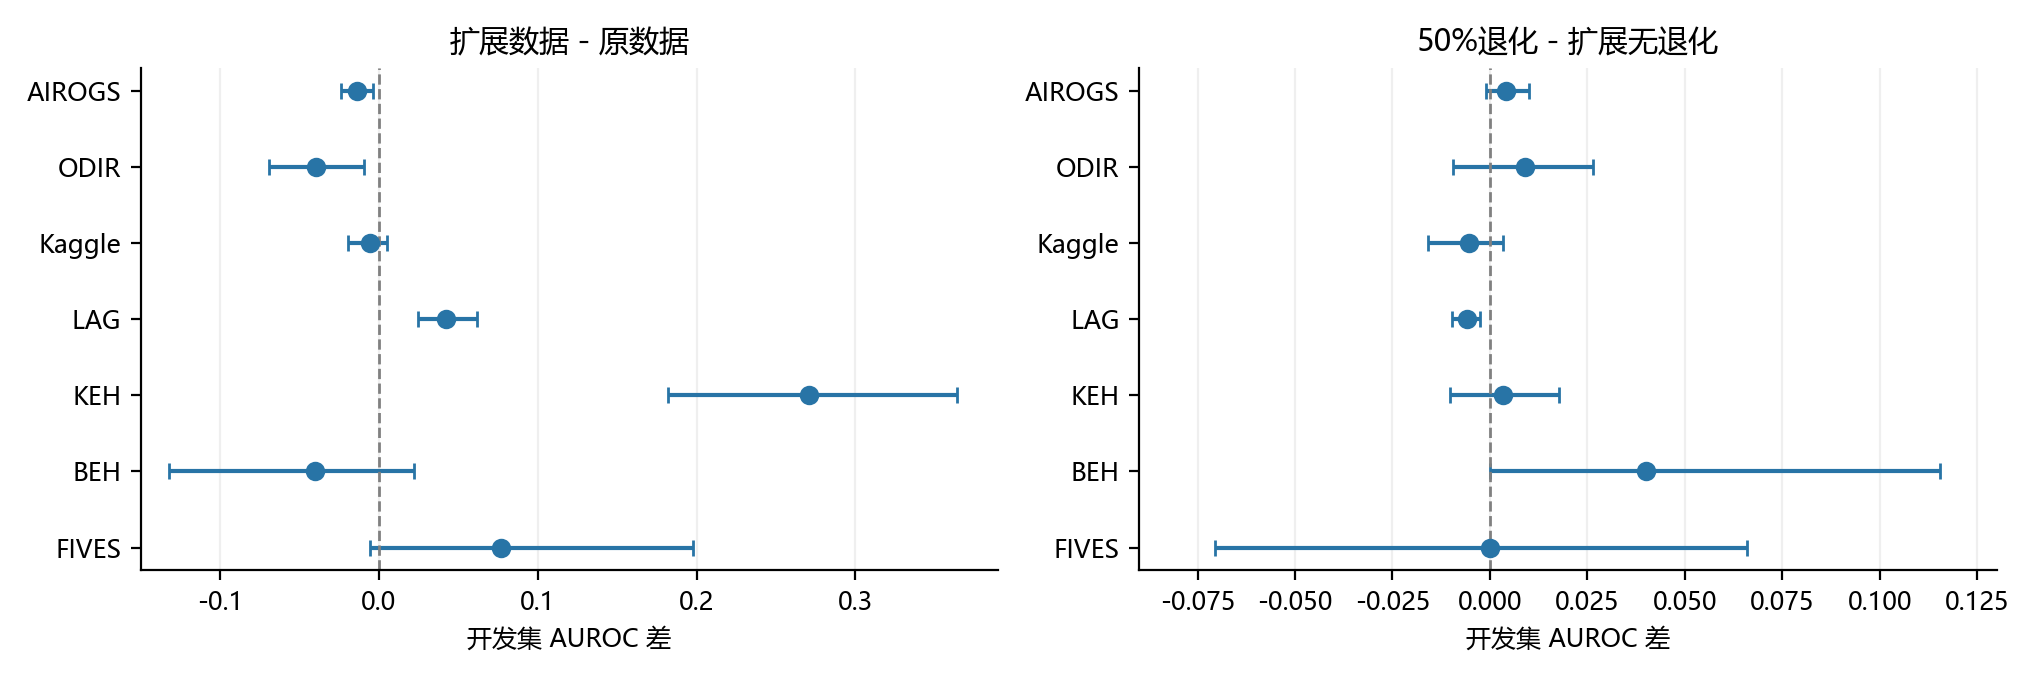
\includegraphics[keepaspectratio,alt={第1,200次更新权重的来源AUROC配对差异}]{source-differences.zh.png}}
\caption{第1,200次更新权重的来源AUROC配对差异}
\end{figure}

图1左侧比较扩展无退化与原数据，右侧比较 50\% 退化与扩展无退化。圆点是
AUROC 差，横线是关联组重采样的 95\%
区间，虚线是零差异。左右横轴范围不同，以便看清各自的变化。50\% 退化在
LAG 原图上下降 0.0058，区间为 {[}−0.0098, −0.0025{]}；AIROGS、ODIR、KEH
的额外变化区间均覆盖零。

AUPRC
是精确率---召回率曲线下面积，关注阳性检出的精确率和覆盖程度，随来源的阳性比例变化，适合在同来源内比较模型。Brier
分数是预测概率与 0/1 标签之间的平均平方误差，越低表示概率预测越准确。

\Needspace{12\baselineskip}
\begin{longtable}[]{@{}lrr@{}}
\toprule\noalign{}
第1,200次更新，扩展－原数据 & AUPRC差及95\%区间 & Brier差及95\%区间 \\
\midrule\noalign{}
\endhead
\bottomrule\noalign{}
\endlastfoot
AIROGS & -0.0123 {[}-0.0231, -0.0023{]} & +0.0230 {[}+0.0110,
+0.0356{]} \\
ODIR & -0.1604 {[}-0.2920, +0.0104{]} & +0.0217 {[}+0.0027,
+0.0412{]} \\
LAG & +0.0735 {[}+0.0404, +0.1118{]} & -0.0571 {[}-0.0811, -0.0330{]} \\
KEH & +0.2578 {[}+0.1561, +0.3600{]} & -0.1482 {[}-0.1998, -0.0973{]} \\
\end{longtable}

KEH 和 LAG 的 AUPRC 提高、Brier 下降，AIROGS 的 AUPRC 下降、Brier
上升，与 AUROC 的方向一致。ODIR 的 Brier 上升，但 AUPRC
差异区间覆盖零。ODIR 的 305 张开发图像只有 193 个关联组，其中阳性组 19
个，这使阳性检出指标的区间较宽。

\subsection{新增来源如何改变采样和权重选择}\label{ux65b0ux589eux6765ux6e90ux5982ux4f55ux6539ux53d8ux91c7ux6837ux548cux6743ux91cdux9009ux62e9}

每次优化更新使用一批采样图像；同一张图像可在训练过程中出现多次。现有采样器为每张图像分配其``来源与类别组合''图像数的平方根倒数权重。一个组合内图像越多，其总采样权重越大，但增长慢于图像数。加入新来源后，旧来源分得的采样比例降低。

\Needspace{12\baselineskip}
\begin{longtable}[]{@{}lrr@{}}
\toprule\noalign{}
方案 & 原数据采样次数／不同原图 & 新增数据采样次数／不同原图 \\
\midrule\noalign{}
\endhead
\bottomrule\noalign{}
\endlastfoot
原数据 & 19,186/8,339 & 0/0 \\
扩展数据 & 9,484/5,929 & 9,708/3,901 \\
30\%退化 & 9,484/5,929 & 9,708/3,901 \\
50\%退化 & 9,484/5,929 & 9,708/3,901 \\
\end{longtable}

表中``不同原图''表示实际至少采样过一次的图像。原数据对照共采样 19,186
次，覆盖 8,339/10,338 张训练图像（80.7\%）。扩展方案中，原数据采样 9,484
次，占 49.4\%，覆盖 5,929 张原图（57.4\%）；新增数据采样 9,708 次，占
50.6\%，覆盖 3,901/5,142
张新增训练图像（75.9\%）。三个扩展方案逐图采样次数完全相同，适合比较退化增强的影响。末尾不满批次使原数据与扩展方案的总采样次数相差
6 次。

新增图像最多重复 30 次，原数据对照最多重复 14
次。数据扩展同时改变了来源组成、原数据采样次数和重复频率；下一轮控制原数据采样配额，可以进一步检验这些因素对原来源表现的影响。

\begin{figure}[H]
\centering
\pandocbounded{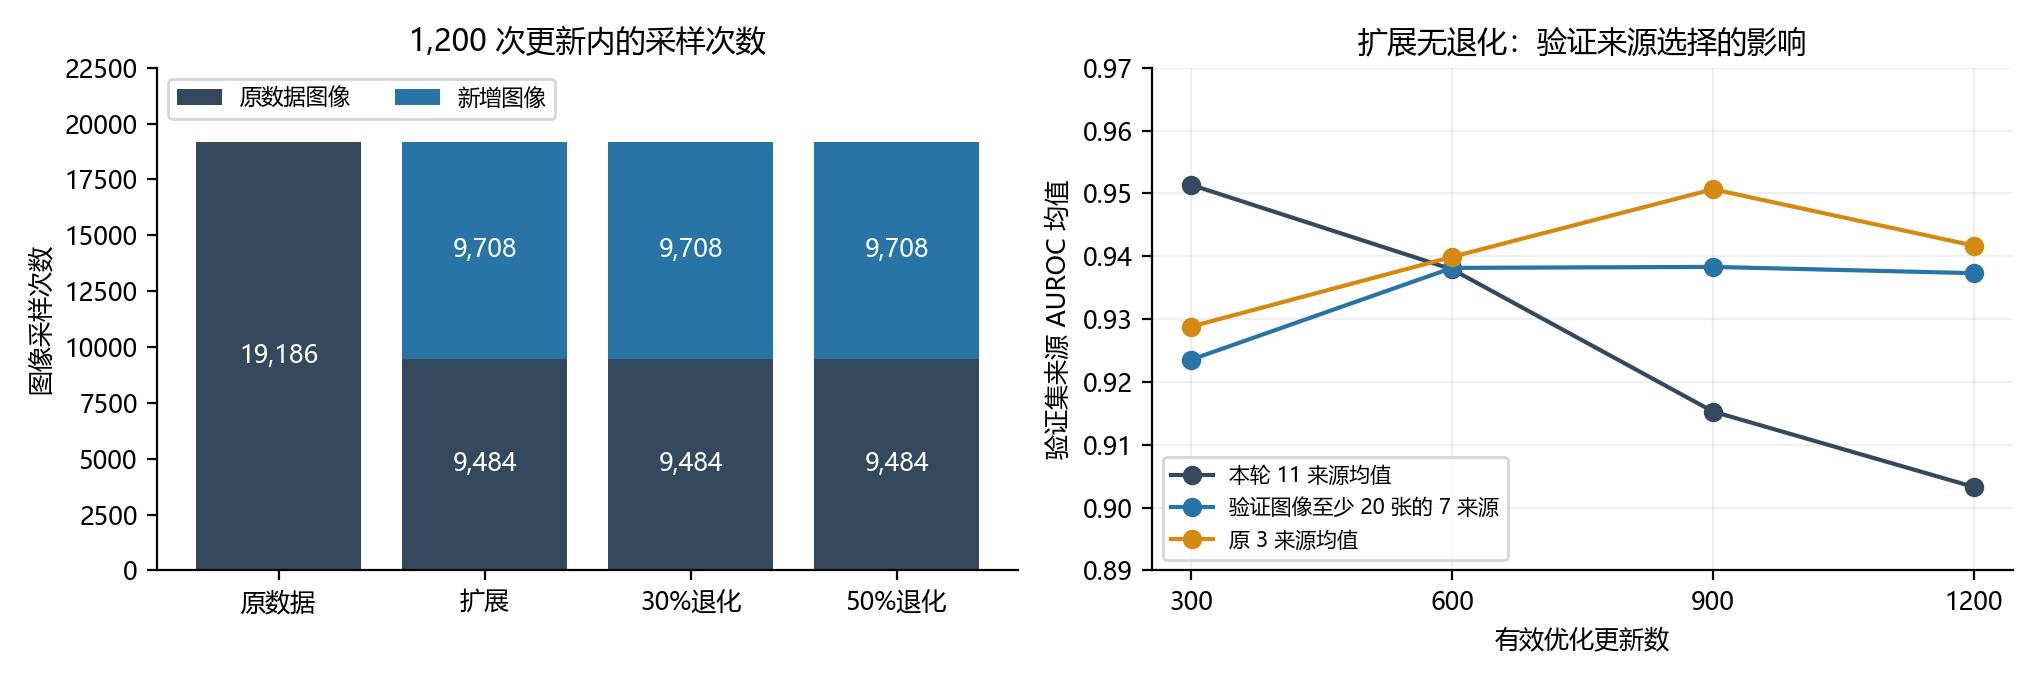
\includegraphics[keepaspectratio,alt={实际图像采样次数与验证指标变化}]{exposure-selection.zh.png}}
\caption{实际图像采样次数与验证指标变化}
\end{figure}

图2左侧显示四组的原数据和新增数据采样次数；右侧显示扩展无退化方案在三种验证来源组合下的
AUROC 等权均值。本轮选择权重时使用 11
个同时包含阳性和阴性的验证来源。HRF、CRFO、Fundus-AVSeg、LES-AV 分别只有
4、6、3、2 张验证图像，合计 15 张，却占这个均值 4/11，即 36.4\% 的权重。

扩展无退化从第 300 到 1,200 次更新，HRF AUROC 从 1.0 降至 0.5，使 11
来源均值下降 0.04545；该均值的总降幅为 0.04807。CRFO 另贡献
−0.01136，其他来源的改善抵消了部分下降。原数据对照中，CRFO 从 0.5 升至
1.0，贡献 +0.04545，而均值总升幅为
0.03241。少量验证图像对权重选择有较大影响。

若分析至少有 20 张验证图像的七个来源，扩展无退化的均值从 0.9235 升至
0.9373，最高点位于第 900 次更新；原三个来源的均值也在第 900
次更新最高。这是对已有验证日志的敏感性分析。第 600 和 900
次更新的完整权重未保存，因此开发集结果仍使用已保存的第 300 和 1,200
次权重。

\subsection{退化增强在合成失焦下的效果}\label{ux9000ux5316ux589eux5f3aux5728ux5408ux6210ux5931ux7126ux4e0bux7684ux6548ux679c}

合成退化评估使用同一组 384 张开发原图，包括阳性 146 张、阴性 238
张，按图像标识的哈希固定选取。失焦半径以 512 像素眼底视野为参照取
2，并随实际视野缩放；曝光变体将亮度乘以
0.70。每张图像的原图与退化版本配对比较。下表使用第 1,200
次更新权重，以预测概率大于 0.5 判为阳性；该阈值用于本轮结果展示。

\Needspace{12\baselineskip}
\begin{longtable}[]{@{}lrrrr@{}}
\toprule\noalign{}
条件／指标 & 原数据 & 扩展数据 & 30\%退化 & 50\%退化 \\
\midrule\noalign{}
\endhead
\bottomrule\noalign{}
\endlastfoot
原图: AUROC & 0.9423 & 0.9690 & 0.9702 & 0.9688 \\
原图: 漏诊／误报 & 30/16 & 23/15 & 21/13 & 23/14 \\
失焦: AUROC & 0.9193 & 0.8894 & 0.9332 & 0.9449 \\
失焦: 漏诊／误报 & 55/10 & 18/68 & 36/23 & 28/19 \\
曝光0.70: AUROC & 0.9382 & 0.9536 & 0.9611 & 0.9564 \\
曝光0.70: 漏诊／误报 & 39/13 & 21/23 & 26/17 & 29/18 \\
\end{longtable}

失焦条件下，50\% 退化相对扩展无退化的 AUROC 增加 0.0555 {[}0.0308,
0.0817{]}，AUPRC 增加 0.1019 {[}0.0511, 0.1592{]}，Brier 下降 0.0684
{[}0.0445, 0.0938{]}。误报从 68/238 降至 19/238，误报率下降 20.59
个百分点 {[}15.25, 26.03{]}；漏诊从 18/146 升至 28/146，漏诊率增加 6.85
个百分点 {[}0.71,
13.33{]}。排序改善与固定阈值下的漏诊---误报变化需要一起评价。

\begin{figure}[H]
\centering
\pandocbounded{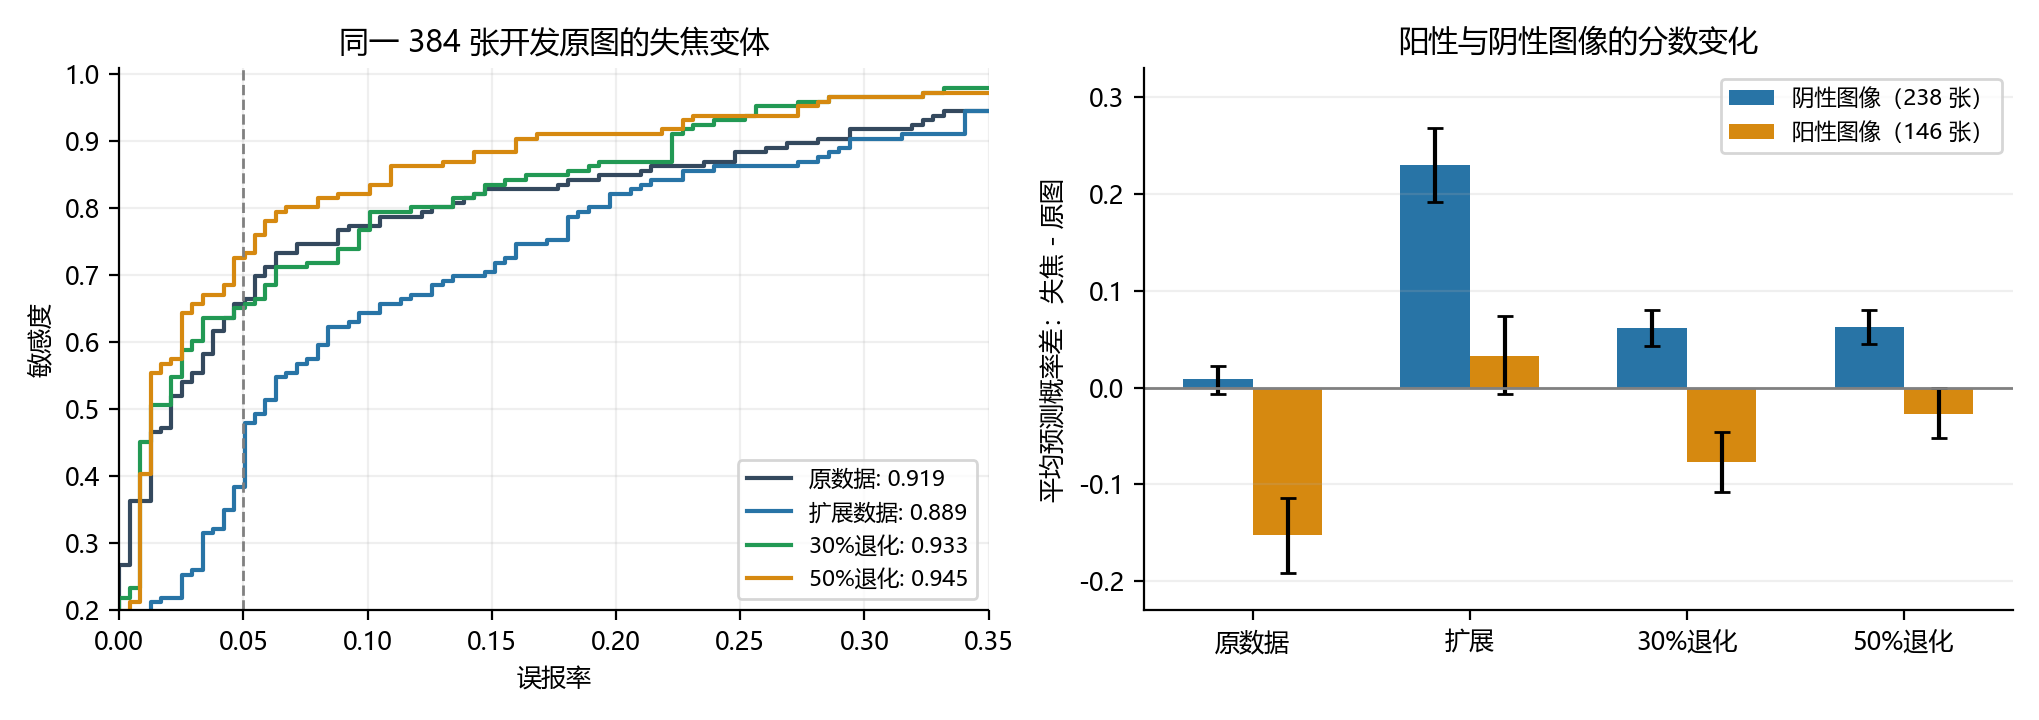
\includegraphics[keepaspectratio,alt={合成失焦下的ROC曲线与预测概率变化}]{defocus-ranking-shifts.zh.png}}
\caption{合成失焦下的ROC曲线与预测概率变化}
\end{figure}

图3左侧的 ROC 曲线展示不同阈值对应的敏感度与误报率，图例同时标出
AUROC；右侧按真实标签显示失焦分数减去原图分数的平均差及 95\%
区间。扩展无退化的阴性图像分数平均增加 0.2295，50\% 退化只增加
0.0622。原数据对照的阳性分数平均下降 0.1523，50\% 退化下降
0.0273。退化增强减轻了失焦对阳性和阴性分数的影响。

将同一退化子集上的特异度匹配到 95.4\% 后，四组失焦敏感度分别为
65.8\%、38.4\%、65.1\%、72.6\%。这项探索性比较为每组、每种条件重新计算阈值，用来解释排序表现。来源内比较也显示改善：50\%
退化在失焦 AIROGS 上的 AUROC 增加 0.0691 {[}0.0258, 0.1149{]}，在 LAG
上增加 0.0835 {[}0.0341, 0.1455{]}。

另一项比较固定每组从原始验证阴性图像设定的来源阈值，再用于原图与退化版本。验证集同时包含两类标签的七个来源贡献
356 张压力评估图像，其中阳性 139 张、阴性 217 张；其余 28
张图像所在的小来源缺少两类验证标签。下表依次列出漏诊数／误报数。

\Needspace{12\baselineskip}
\begin{longtable}[]{@{}lrrrr@{}}
\toprule\noalign{}
条件：验证阈值固定 & 原数据 & 扩展数据 & 30\%退化 & 50\%退化 \\
\midrule\noalign{}
\endhead
\bottomrule\noalign{}
\endlastfoot
原图 & 34/11 & 27/7 & 30/10 & 30/11 \\
失焦 & 63/10 & 28/47 & 45/16 & 40/10 \\
曝光0.70 & 38/8 & 25/15 & 30/13 & 35/13 \\
\end{longtable}

固定验证阈值后，50\% 退化相对扩展无退化的失焦误报从 47 降至 10，漏诊从
28 升至 40。曝光乘以 0.70 时，AUROC 差为 +0.0028 {[}−0.0078,
0.0138{]}，漏诊从 25 升至
35。当前增强收益主要集中在失焦；下一轮单独比较失焦增强与混合增强，可以确定有效的退化类型和强度。

\subsection{真实低质量图像的检出与标签分布}\label{ux771fux5b9eux4f4eux8d28ux91cfux56feux50cfux7684ux68c0ux51faux4e0eux6807ux7b7eux5206ux5e03}

真实低质量开发图像来自 FIVES 7 张、MSHF 5 张，均为阳性，属于 12
个不同关联组。在阈值 0.5 下，原数据对照检出 7/12，三个扩展方案均检出
12/12。12/12 对应的精确二项 95\% 区间为 73.5\%--100\%；FIVES 和 MSHF
分别为 59.0\%--100\% 和 47.8\%--100\%。新增检出为 FIVES 2 张、MSHF 3
张，无新增漏诊；比较同图检出变化的 McNemar 精确检验双侧
p=0.0625。区间说明这组图像的检出比例仍存在较大的抽样不确定性。

\begin{figure}[H]
\centering
\pandocbounded{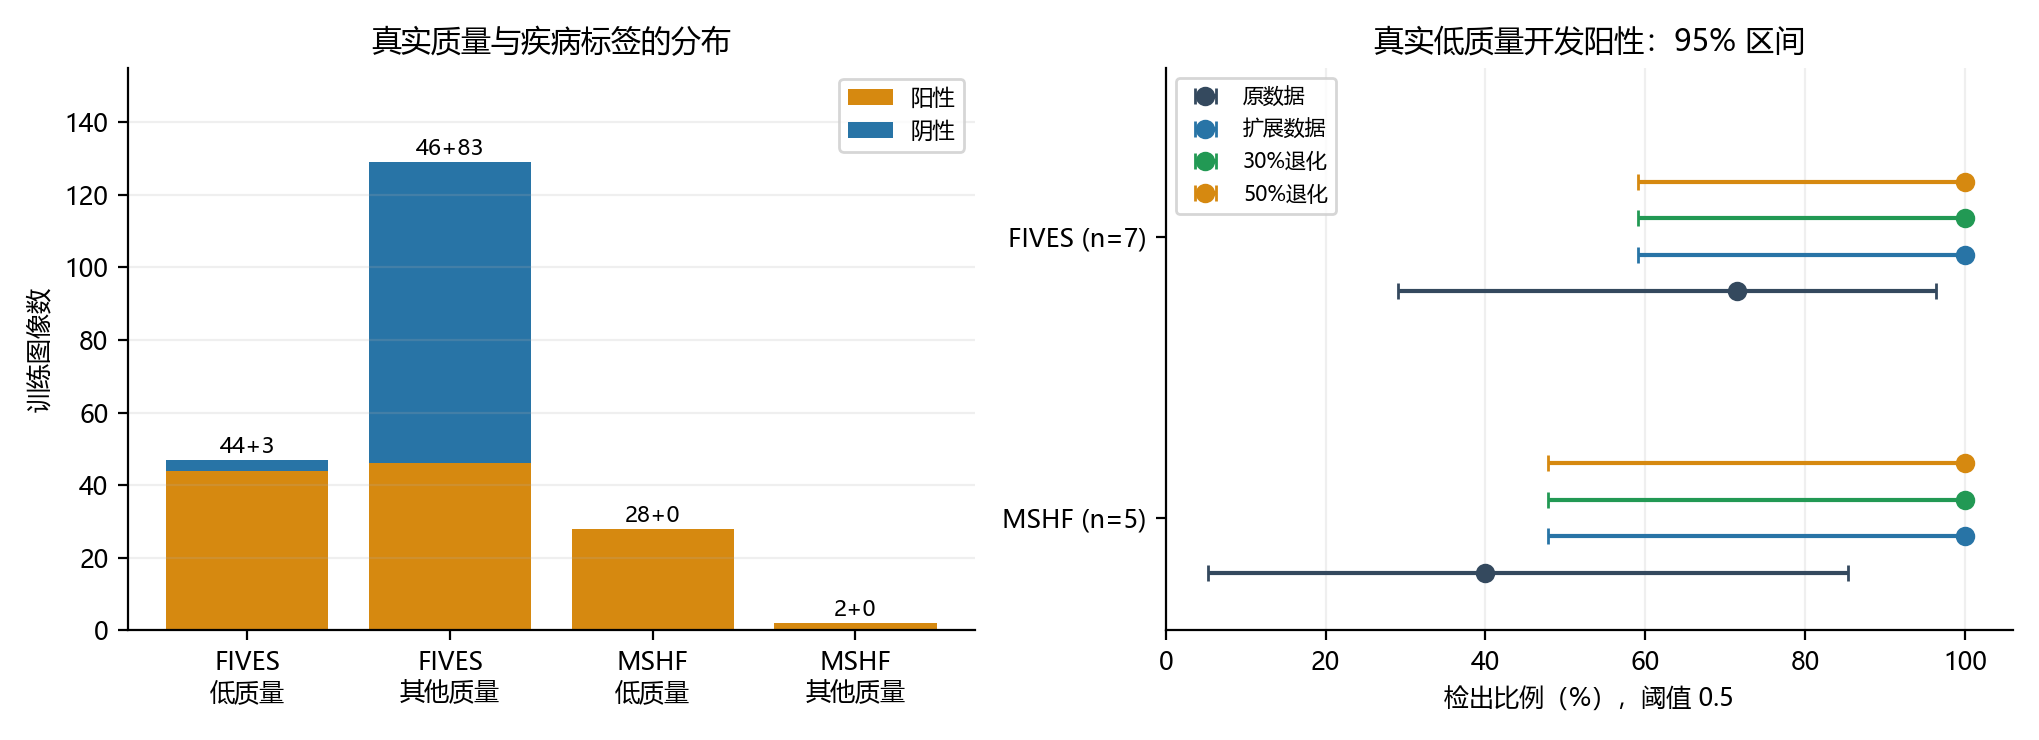
\includegraphics[keepaspectratio,alt={真实质量与疾病标签的训练分布以及开发阳性检出比例}]{real-quality-labels.zh.png}}
\caption{真实质量与疾病标签的训练分布以及开发阳性检出比例}
\end{figure}

图4左侧按来源和原始质量标注显示训练图像数，柱顶数字依次为阳性数＋阴性数；右侧显示同来源真实低质量开发阳性的检出比例与精确二项
95\% 区间。FIVES 以至少一个质量维度标为差定义低质量，MSHF
使用总体质量标注。``其他质量''包含该来源剩余质量档次，两个来源保留各自的标注标准。

FIVES 的 47 张低质量训练图像中，阳性 44 张、阴性 3 张；其他 129
张中，阳性 46 张、阴性 83 张。MSHF 的 28 张低质量和 2
张其他质量训练图像全部为阳性。实际训练采样中，这两个来源的真实低质量阳性出现
413 次，阴性仅 10
次。质量与疾病标签高度关联，因此下一轮应加入同来源真实低质量阴性，比较质量平衡采样，区分来源、质量线索与疾病特征的作用。

固定验证来源阈值后，扩展无退化和 50\% 退化均检出 FIVES 的 7/7
张低质量阳性。对比这两个方案，FIVES 全部 13 张开发阳性的敏感度从 76.9\%
升至 92.3\%，14 张阴性的特异度从 100\% 降至 78.6\%。阈值来自 14
张验证阴性，并取其最高分数，后续需要更多阴性图像来稳定阈值。MSHF
当前仅有阳性图像，其来源内特异度需在补充阴性后评估。

\subsection{下一轮控制实验建议}\label{ux4e0bux4e00ux8f6eux63a7ux5236ux5b9eux9a8cux5efaux8bae}

建议设置一个原数据对照，以及四个扩展方案，分别组合两种采样方法（现有方法、原数据
65\% 采样配额）和两种增强设置（无退化、50\%
混合退化）。每组使用三个共同种子、相同初始化条件和 2,400
次有效更新。按每批 16 张计算，65\% 配额预计提供 24,960
次原数据采样，高于本轮原数据对照的 19,186
次；来源内继续使用平方根倒数权重。在相同预算下比较采样与增强，并保存第
1,200 和 2,400 次更新权重，评估继续训练的影响。

预先指定 AIROGS、ODIR、Kaggle、LAG、KEH 五来源 AUROC
的等权均值作为主要权重选择指标，同时报告原三个来源均值、各来源敏感度和特异度。BEH、FIVES
和更小来源作为补充评估。每 300
次更新保存完整权重与预测，分别报告开发图像重采样区间和跨训练种子的变化。

随后在相同应用概率、采样序列和更新预算下，比较单独失焦与混合退化增强。评估固定验证阈值下的漏诊、误报、真实低质量阴性表现，以及原图
AUROC 和
Brier。依据预先约定的原来源表现、质量分层结果和复核工作量选择模型与阈值，再执行最终测试。上述方案是下一轮建议，尚未运行。

\subsection{分析产物与复现}\label{ux5206ux6790ux4ea7ux7269ux4e0eux590dux73b0}

\href{../training-results/training-results.zh.md}{训练结果} ·
\href{../training-results/data-audit.zh.md}{数据审计} ·
\href{../training-results/degradation-audit.zh.md}{退化审计} ·
\href{training-exposure.json}{图像采样记录} ·
\href{figure-data.json}{图表数据} ·
\href{../../../../tools/analyze_expansion_results_20261113.py}{分析程序}
·
\href{../../../../tools/report_expansion_analysis_20261113.py}{报告生成程序}

在训练环境运行分析程序的 \texttt{-\/-extract-draws}
选项，提取检查点内的逐图采样计数；随后在文档环境运行分析程序和报告生成程序。分析核对四组的图像标识、标签、来源、关联组与冻结清单，并记录输入文件的
SHA256。统计测试覆盖并列分数处理、关联组重采样和同图配对检查。

\end{document}
